\documentclass[slovene,11pt,a4paper]{article}
%\usepackage{fullpage}
\usepackage[margin=2cm]{geometry}

\usepackage[T1]{fontenc}



%dodatni paketki:
\usepackage{graphicx}
\usepackage{amsmath,amsfonts,amsthm} %matematicni paket
\usepackage{color} % omogoča barvno pisanje
\usepackage[utf8]
{inputenc}
\usepackage[slovene]{babel} % slovenski jezik/hyphenation
\usepackage{hyperref} %naredi vse povezave rečerenc, kazala,...
\numberwithin{equation}{section} % Number equations within sections (i.e. 1.1, 1.2, 2.1, 2.2 instead of 1, 2, 3, 4)
\numberwithin{figure}{section} % Number figures within sections (i.e. 1.1, 1.2, 2.1, 2.2 instead of 1, 2, 3, 4)
\numberwithin{table}{section} % Number tables within sections (i.e. 1.1, 1.2, 2.1, 2.2 instead of 1, 2, 3, 4)
\usepackage{eurosym} %za znak €

\usepackage{mathrsfs}
\usepackage{mathabx} % za kemisjke smeri in naslednje 3 vstrice
\catcode`_=12
\begingroup\lccode`~=`_\lowercase{\endgroup\let~\sb}
\mathcode`_="8000


\usepackage[margin=2cm]{geometry}



\begin{document}
\begin{titlepage}

\newcommand{\HRule}{\rule{\linewidth}{0.5mm}} % Defines a new command for the horizontal lines, change thickness here

\center % Center everything on the page

%----------------------------------------------------------------------------------------
%	LOGO
%----------------------------------------------------------------------------------------

%\includegraphics{Logo}\\[1cm] % Include a department/university logo - this will require the graphicx package
 
%----------------------------------------------------------------------------------------


\includegraphics[width=2cm]{slike/aaa}\\[0.5cm]
 
%----------------------------------------------------------------------------------------
%	NASLOV DELA
%----------------------------------------------------------------------------------------
\textit{Univerza v Ljubljani}\\
\textit{Fakulteta za {\color{red}matematiko in fiziko}}\\[0.5cm]

\emph{Oddelek za fiziko}\\[0.5cm] % Oddelek za fiziko


%----------------------------------------------------------------------------------------
%	TITLE SECTION
%--------------------------------------------------------------------------------------
\HRule \\[0.4cm]
\huge {\bfseries 12. naloga: - - Spektralna analiza in filtriranje}\\[0.4cm] % NASLOV SEMINARJA
\HRule \\[0.5cm] 

 \textsc{\large Poročilo pri predmetu modelska analiza 1}\\
 \textsc{\large 2015/2016}\\[1cm] % SEMINASKO DELO
 
%----------------------------------------------------------------------------------------
%	AUTHOR SECTION
%----------------------------------------------------------------------------------------



% If you don't want a supervisor, uncomment the two lines below and remove the section above
\Large \emph{Avtor:}\\
Klemen \textsc{Rahne}\\
28152028\\[2cm]
%----------------------------------------------------------------------------------------
%	DATUM
%----------------------------------------------------------------------------------------

{\large \today } \\[0.5cm] % Date, change the \today to a set date if you want to be precise

	

\end{titlepage}


%----------------------------------------------------------------------------------------
%	KAZALO
%----------------------------------------------------------------------------------------

%\tableofcontents

%----------------------------------------------------------------------------------------
%	ZAČETEK TEKSTA
%----------------------------------------------------------------------------------------


\section{Frekvenčni sprekter}
Iz datotek, dosegljivih na spletni strani moramo določiti frekvenčni speketer. To dosešemo s Fourierovo transformacijo:
\begin{equation}
\mathcal{F}_k= \frac{1}{N} \sum_{j=1}^N f_j e^{\frac{- ik j 2\pi}{N}}
\end{equation}
kjer je $f_k$ izmerjena funkcija.


\begin{figure}[h]
\centering
\begin{minipage}{0.5\textwidth}
\centering
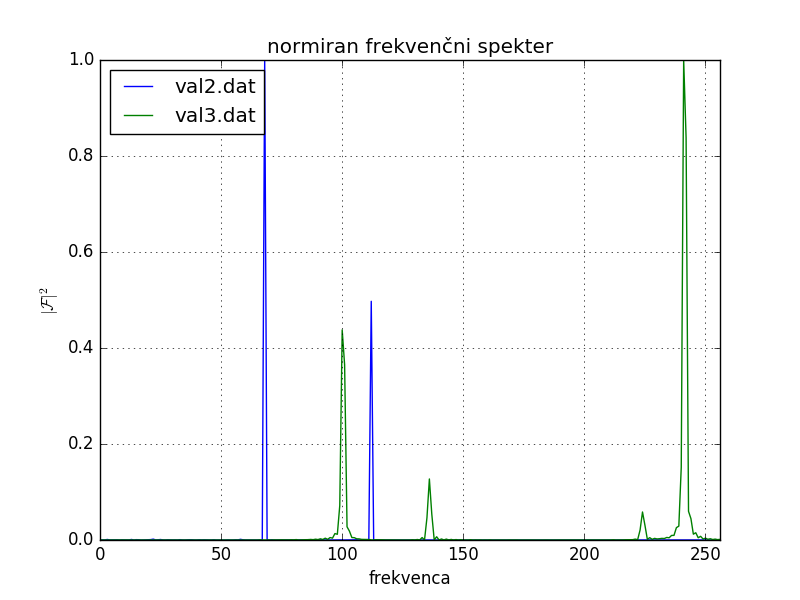
\includegraphics[scale=0.4]{slike/prva_naloga_1.png}
%\caption{first figure}
\end{minipage}\hfill
\begin{minipage}{0.5\textwidth}
\centering
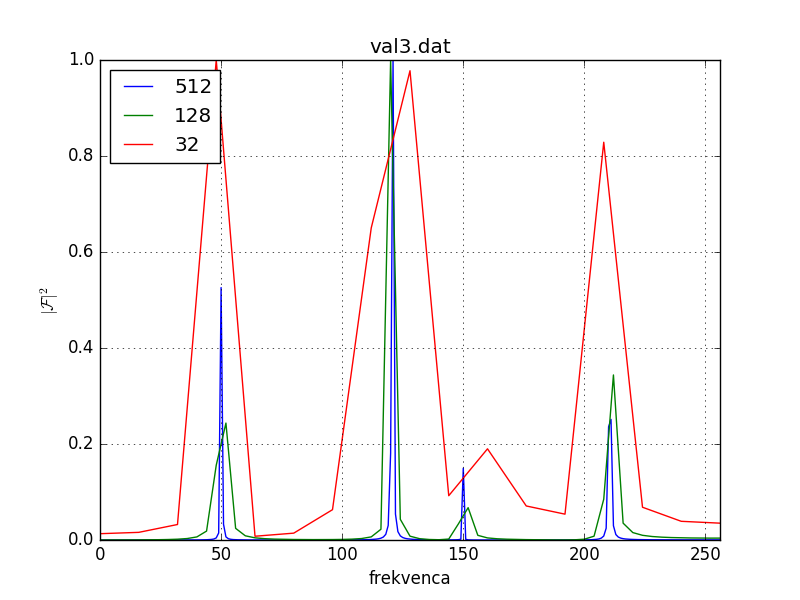
\includegraphics[scale=0.4]{slike/prva_naloga_2.png}
%\caption{second figure}
\end{minipage}
\caption{Na levi imamo normirana frekvenčna spektra iz datotek $val2.dat$ in $val3.dat$. Na desni imamo primerjavo spektra iz datoteke $val3.dat$, pri različnih intervalih Fourierove transformacije. Opazimo, da se širina ostrega širina frekvenčnega vrha veča. }
\end{figure}

Pri diskretni Fourierovi transformaciji prihaja do dveh problemov: 1.) potujitev in 2.) puščanje. Puščanje odpravimo s ti. okenskimi funkcijami. Našo Fourierovo transformacijo modificiramo:

\begin{equation}
\mathcal{F}_k= \frac{1}{N} \sum_{j=1}^N w_j f_j e^{\frac{- ik j 2\pi}{N}}
\end{equation}
kjer je $w_k$ vrednost okenske funkcije. Okenske funkcije imajo v $N/2$ praviloma vrednost $1$, ter nato vrednost pada proti $0$.

\begin{figure}[h]
\centering
\begin{minipage}{0.5\textwidth}
\centering
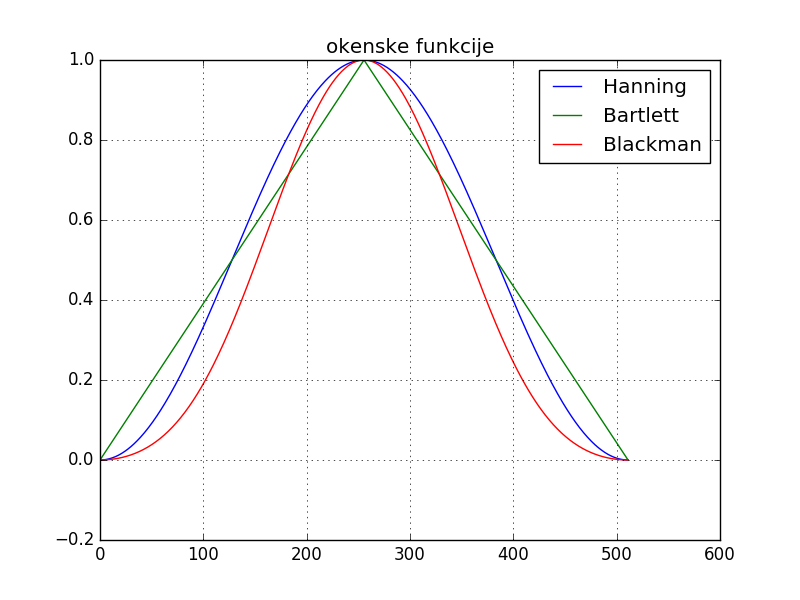
\includegraphics[scale=0.4]{slike/prva_naloga_okenske_funkcije.png}
%\caption{first figure}
\end{minipage}\hfill
\begin{minipage}{0.5\textwidth}
\centering
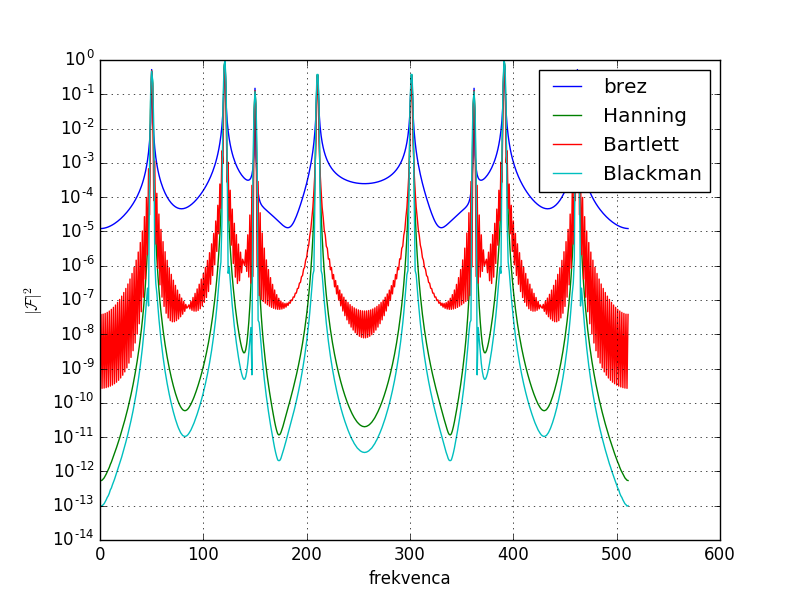
\includegraphics[scale=0.4]{slike/prva_naloga_okenske.png}
%\caption{second figure}
\end{minipage}
\caption{Na levi imamo primere okenskih funkcij, ki smo jih uporabili na podatkih iz datoteke $val3.dat$-na desni. Opazimo, da s uporabo "najslabše" okenske funkcije (Bartlee-preprost trikotnik) izboljšamo frekvenčni spekter 2 velikostna razreda, s še boljšo okensko funkcijo tudi za 4 ali več velikostih razredov.}
\end{figure}

\section{Wienerjev filter}

Za rekonstrukcijo vhodnega signala, ki se zaradi odzivne funkcije sistema in šuma spremeni:
\begin{equation*}
c(t)=u(t)*r(t)+n(t)=s(t)+n(t)
\end{equation*}
kjer je $c(t)$ izmerjen signal, $u(t)$ vhodni signal, ki ga ne pozanmo, $r(t)$ odzivna funkcija sistema ter $n(t)$ šum. N. Wiener je za izračun vhodnega signal $u(t)$ predlagal, da se pred dekonvolucijo funkcijo $\mathcal{U}(f)=\frac{\mathcal{C}(f)}{R(f)}$ pomnoži s funkcijo:
\begin{equation}
\Phi=\frac{|\mathcal{S}(f)|^2}{|\mathcal{S}(f)|^2+|\mathcal{N}(f)|^2}
\end{equation}
Pri tem so vse funkcije z veliko samo Fourierovo transformacijo funkcij s malo črko. Ker ne poznamo kašen je šum ga ocenimo.




\begin{figure}[h]
\centering
\begin{minipage}{0.5\textwidth}
\centering
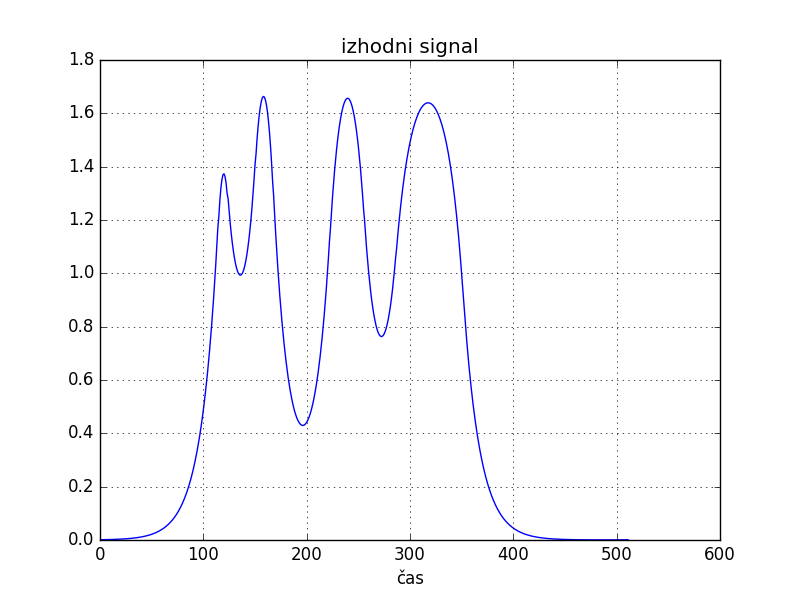
\includegraphics[scale=0.4]{slike/druga_izhodni_signal.png}
%\caption{first figure}
\end{minipage}\hfill
\begin{minipage}{0.5\textwidth}
\centering
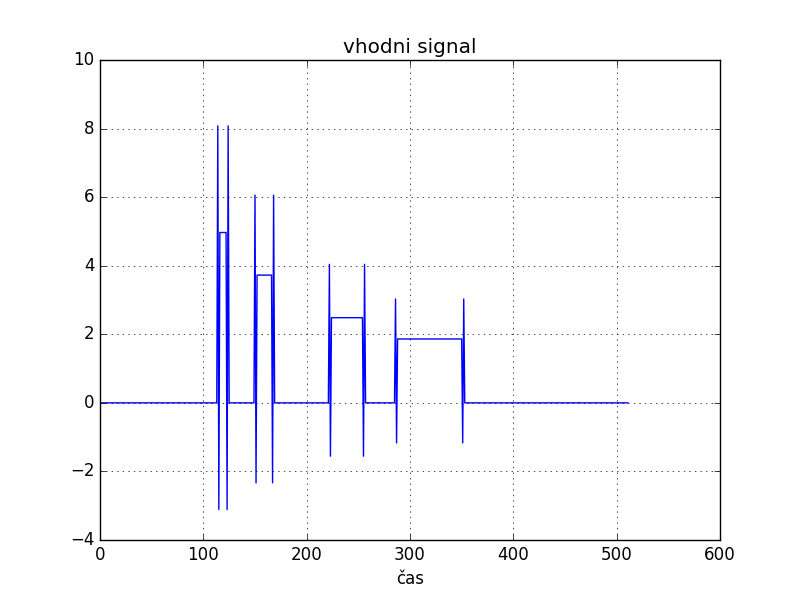
\includegraphics[scale=0.4]{slike/druga_vhodni_signal.png}
%\caption{second figure}
\end{minipage}
\caption{Na levi imamo naš izmerjeni signal, desni pa njena dekompozicija. Prenosna funkcija je $r(t)=\frac{1}{2 \tau}e^{-\frac{t}{\tau}}$, $\tau=16$. Tu je $\Phi=1$, saj tu ni šuma.}
\end{figure}




\begin{figure}[h]
\centering
\begin{minipage}{0.5\textwidth}
\centering
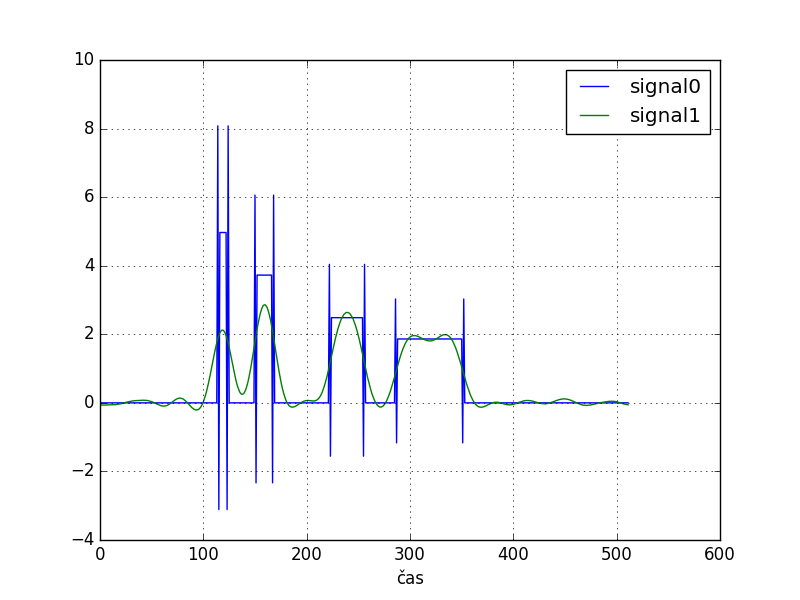
\includegraphics[scale=0.4]{slike/druga_delna_rezultati.png}
%\caption{first figure}
\end{minipage}\hfill
\begin{minipage}{0.5\textwidth}
\centering
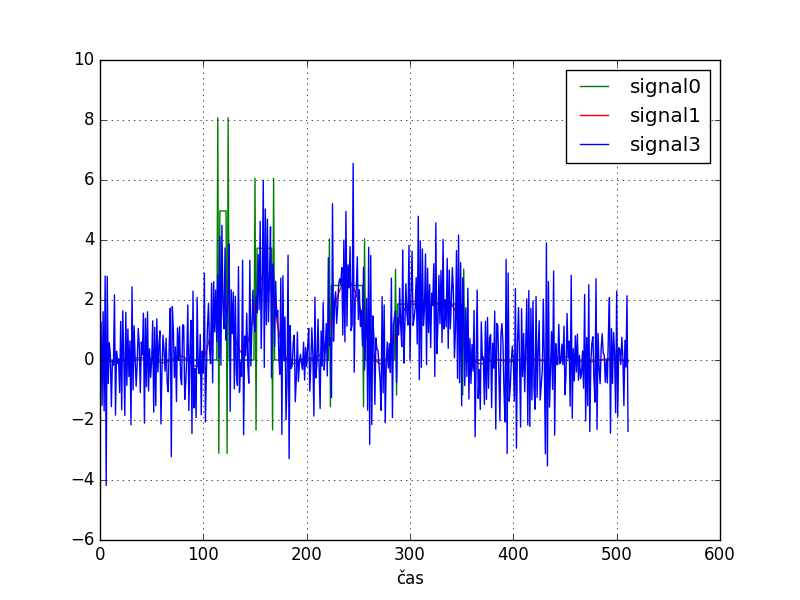
\includegraphics[scale=0.4]{slike/druga_delna_rezultati3.png}
%\caption{second figure}
\end{minipage}
\caption{Na levi imamo primerjavo signala brez šuma s signalom, ki ima malo šuma. N desni imamo v treti krivulji še več šuma. Oblika še priblišno sledi krivulji brez šuma.}
\end{figure}


\begin{figure}[h]
\centering
\begin{minipage}{0.5\textwidth}
\centering
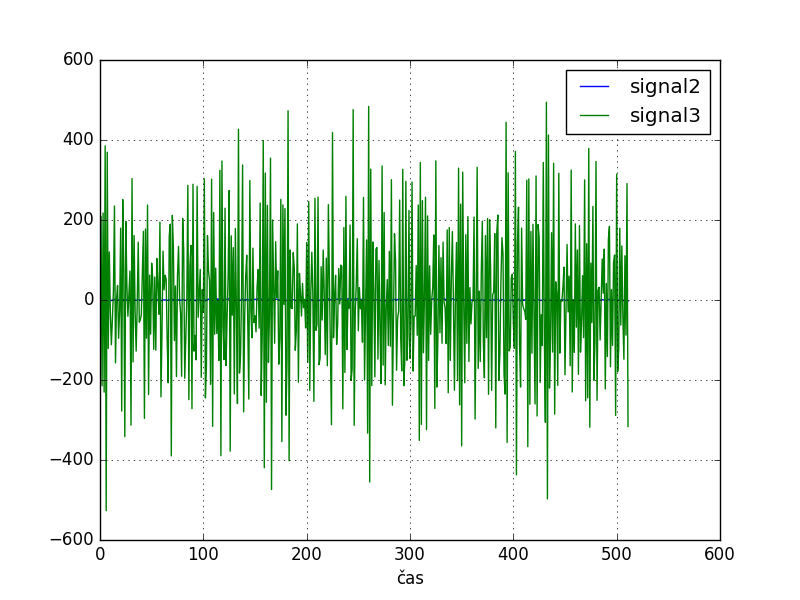
\includegraphics[scale=0.4]{slike/druga_delna_rezultati2.png}
%\caption{first figure}
\end{minipage}\hfill
\begin{minipage}{0.5\textwidth}
\centering
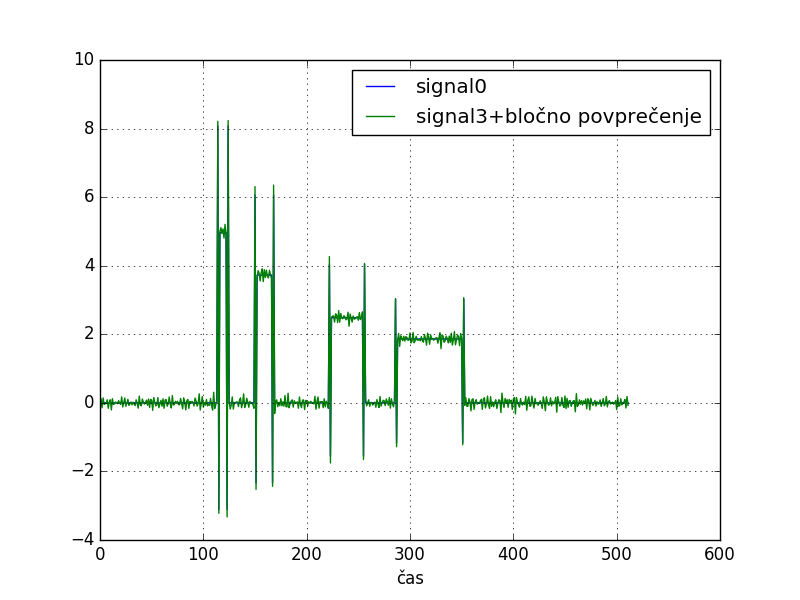
\includegraphics[scale=0.4]{slike/12_2_blocno_popvprecenje.png}
%\caption{second figure}
\end{minipage}
\caption{Na levi, zelena krivulja je rekonstrukcija iz datoteke $signal3.dat$. V izvorni datoteki, je že toliko šuma, da tudi Wienerjev filter ne prinese izboljšave. Zato smo poskusili s ti. bločno povprečenje. V izvorni datoteki smo povprečili podatke v blokih po $20$ točk. S tem smo izgubili $20$ točk, vendar smo začetnih in kočnih $10$ točk, kar enačili s povprečjem prvih/zadnjih deset točk. Izboljšava je očtina, saj se oblika skoraj ujema s obliko, ko ni nič šuma.}
\end{figure}

\pagebreak
\section{Lincolnova slika}
Oglejmo si kako izgledajo dekonvolirane slike iz datotek $lincoln\_L30\_N{00,10,20,30}$:

\begin{figure}[h]
\centering
\begin{minipage}{0.5\textwidth}
\centering
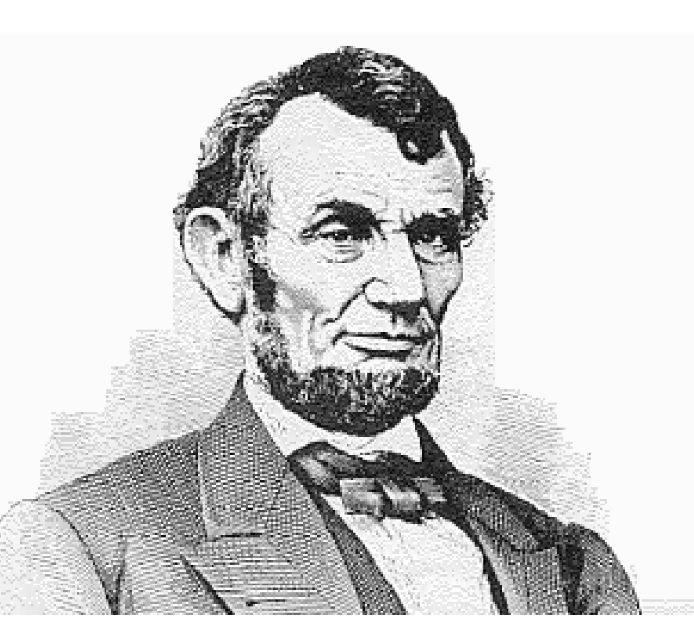
\includegraphics[scale=0.4]{slike/lincon1.png}
%\caption{first figure}
\end{minipage}\hfill
\begin{minipage}{0.5\textwidth}
\centering
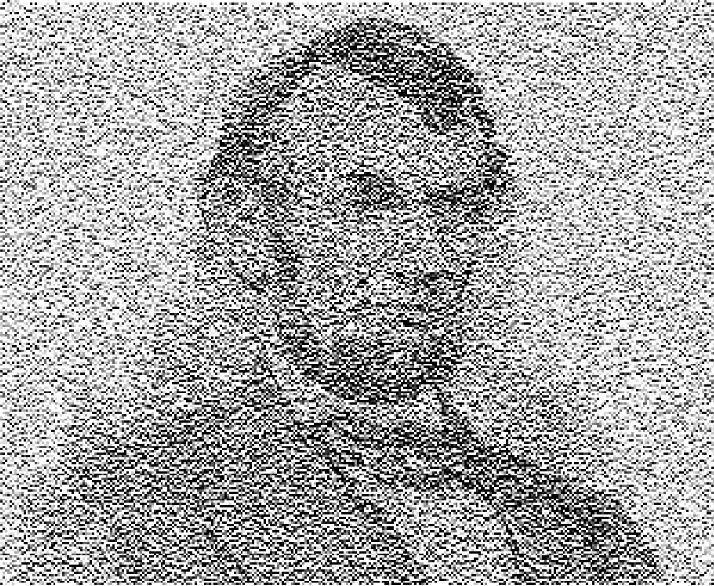
\includegraphics[scale=0.4]{slike/lincon2.png}
%\caption{second figure}
\end{minipage}
\caption{Na levi je preprosta dekonvolucija slike brez šuma, na desni pa vsebuje nekaj šuma. Prenosna funkcija sistema je $r(t)=\frac{1}{\tau}e^{-\frac{t}{\tau}}$, $\tau=30$}
\end{figure}



\end{document}
